\documentclass[hidelinks,12pt]{article}
\usepackage[left=0.25cm,top=1cm,right=0.25cm,bottom=1cm]{geometry}
%\usepackage[landscape]{geometry}
\textwidth = 20cm
\hoffset = -1cm
\usepackage[utf8]{inputenc}
\usepackage[spanish,es-tabla, es-lcroman]{babel}
\usepackage[autostyle,spanish=mexican]{csquotes}
\usepackage[tbtags]{amsmath}
\usepackage{nccmath}
\usepackage{amsthm}
\usepackage{amssymb}
\usepackage{mathrsfs}
\usepackage{graphicx}
\usepackage{subfig}
\usepackage{caption}
%\usepackage{subcaption}
\usepackage{standalone}
\usepackage[outdir=./Imagenes/]{epstopdf}
\usepackage{siunitx}
\usepackage{physics}
\usepackage{color}
\usepackage{float}
\usepackage{hyperref}
\usepackage{multicol}
\usepackage{multirow}
%\usepackage{milista}
\usepackage{anyfontsize}
\usepackage{anysize}
%\usepackage{enumerate}
\usepackage[shortlabels]{enumitem}
\usepackage{capt-of}
\usepackage{bm}
\usepackage{mdframed}
\usepackage{relsize}
\usepackage{placeins}
\usepackage{empheq}
\usepackage{cancel}
\usepackage{pdfpages}
\usepackage{wrapfig}
\usepackage[flushleft]{threeparttable}
\usepackage{makecell}
\usepackage{fancyhdr}
\usepackage{tikz}
\usepackage{bigints}
\usepackage{menukeys}
\usepackage{tcolorbox}
\tcbuselibrary{breakable}
\usepackage{scalerel}
\usepackage{pgfplots}
\usepackage{pdflscape}
\pgfplotsset{compat=1.16}
\spanishdecimal{.}
\renewcommand{\baselinestretch}{1.5} 
\renewcommand\labelenumii{\theenumi.{\arabic{enumii}})}

\newcommand{\python}{\texttt{python}}
\newcommand{\textoazul}[1]{\textcolor{blue}{#1}}
\newcommand{\azulfuerte}[1]{\textcolor{blue}{\textbf{#1}}}
\newcommand{\funcionazul}[1]{\textcolor{blue}{\textbf{\texttt{#1}}}}

\newcommand{\pderivada}[1]{\ensuremath{{#1}^{\prime}}}
\newcommand{\sderivada}[1]{\ensuremath{{#1}^{\prime \prime}}}
\newcommand{\tderivada}[1]{\ensuremath{{#1}^{\prime \prime \prime}}}
\newcommand{\nderivada}[2]{\ensuremath{{#1}^{(#2)}}}


\newtheorem{defi}{{\it Definición}}[section]
\newtheorem{teo}{{\it Teorema}}[section]
\newtheorem{ejemplo}{{\it Ejemplo}}[section]
\newtheorem{propiedad}{{\it Propiedad}}[section]
\newtheorem{lema}{{\it Lema}}[section]
\newtheorem{cor}{Corolario}
\newtheorem{ejer}{Ejercicio}[section]

\newlist{milista}{enumerate}{2}
\setlist[milista,1]{label=\arabic*)}
\setlist[milista,2]{label=\arabic{milistai}.\arabic*)}
\newlength{\depthofsumsign}
\setlength{\depthofsumsign}{\depthof{$\sum$}}
\newcommand{\nsum}[1][1.4]{% only for \displaystyle
    \mathop{%
        \raisebox
            {-#1\depthofsumsign+1\depthofsumsign}
            {\scalebox
                {#1}
                {$\displaystyle\sum$}%
            }
    }
}
\def\scaleint#1{\vcenter{\hbox{\scaleto[3ex]{\displaystyle\int}{#1}}}}
\def\scaleoint#1{\vcenter{\hbox{\scaleto[3ex]{\displaystyle\oint}{#1}}}}
\def\scaleiiint#1{\vcenter{\hbox{\scaleto[3ex]{\displaystyle\iiint}{#1}}}}
\def\bs{\mkern-12mu}

\newcommand{\Cancel}[2][black]{{\color{#1}\cancel{\color{black}#2}}}


\hypersetup{
    colorlinks=true,
    linkcolor=blue,
    filecolor=magenta,      
    urlcolor=red,
    }


\author{M. en C. Gustavo Contreras Mayén. \texttt{curso.fisica.comp@gmail.com}\\
M. en C. Abraham Lima Buendía. \texttt{abraham3081@ciencias.unam.mx}}
\title{Material de apoyo: Interfaces de desarrollo \\ {\large Curso Física Computacional}}
\date{ }
\begin{document}

\maketitle

\section{Programando con python.}

Para el desarrollo de problemas y ejercicio con \python, ya hemos presentado una referencia básica a la sintaxis y estructuras de control propias del lenguaje.
\par
Cada vez, el código necesario para resolver un problema aumentará de tamaño y el riesgo de errores también se incrementa, si omitimos alguna instrucción o dejamos un bloque sin identar, no cerramos un paréntesis, etc. El trabajo que hemos hecho con \texttt{Jupyter} ha sido muy útil, ya que ha combinado la revisión de un texto que nos enfoca al tema, y a la ejecución de código en \python.

\subsection{Escribiendo el código.}

Un código en \python debe de generarse con el apoyo de un editor de texto, que nos será de utilidad para escribir el conjunto de instrucciones, funciones, módulos, etc. necesarios para nuestro problema.
\par
Los editores de texto normalmente vienen incluidos en Windows, iOS y Linux, van de los básicos como:
\begin{enumerate}[label=\roman*)]
    \item \texttt{vim}.
    \item \texttt{nano}.
    \item \texttt{neovim}.
    \item \texttt{bloc de notas}.
\end{enumerate}

Un editor de texto permite la escritura de las instrucciones, no resalta el texto si se trata de una palabra reservada de \python, o indica si nos falta un paréntisis o llave, por lo que nos daremos cuenta de la omisión o error de dedo al momento de ejecutar el programa.
\begin{figure}[H]
    \centering
    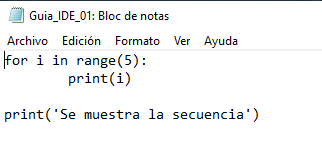
\includegraphics[scale=1]{Imagenes/Guia_IDE_00.png}
    \caption{Un código de \python en el editor de notas de Windows.}
\end{figure}
El archivo con el código en \python{} debe de tener asociada la extensión de archivo \texttt{.py}, para que de esa manera se pueda ejecutar en una terminal.
\par 
Estos editores de texto tienen mejoras cuando se instalan algunos \textit{plugins}, pero esto implica revisar la documentación correspondiente y obtener esa mejora para trabajar el programa.

\subsection{Ejectuando el código.}

Una vez que se ha escrito un código en \python, tenemos un archivo con extensión \texttt{.py}, que para ser ejecutado, se requiere contar con una terminal de nuestra computadora, en Windows puede ser con una ventana de la terminal o Powershell.
\par
Nos debemos de ubicar en la ruta donde se encuentra nuestro archivo, y se ejecuta en la terminal mediante la instrucción:
\begin{center}
\texttt{python nombre\_archivo.py} \quad \keys{\return}
\end{center}

\begin{figure}[H]
    \centering
    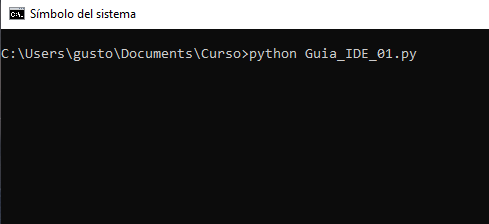
\includegraphics{Imagenes/Guia_IDE_04.png}
    \caption{Ejecutando el archivo en la terminal.}
\end{figure}

En la misma terminal se muestra el resultado que ejecuta el código, siempre y cuando no tengamos algún detalle que interrumpa su proceso.
\begin{figure}[H]
    \centering
    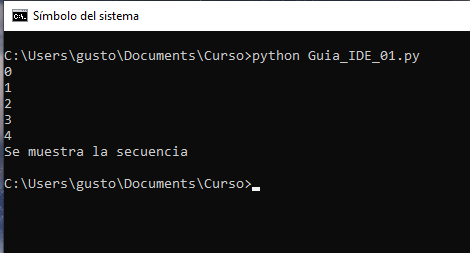
\includegraphics{Imagenes/Guia_IDE_05.png}
    \caption{Resultado del código en la terminal.}
\end{figure}

Cuando estamos comprobando el funcionamiento de un código, cambiar de la aplicación del editor de texto a la terminal, en ocasiones no favorece el trabajo, ya que debemos de intercambiar de aplicaciones por cada vez que hagamos un cambio y queremos ver el resultado en la terminal, veremos en un momento que existen programas llamados \textit{Entornos de Desarrollo Integrados (IDE: Integeated Development Environmet)} que brindarán varias herramientas dentro de una sola aplicación.
\par
Un caso particular de editor de texto y terminal en conjunto es el \textbf{IDLE} que viene integrado en la instalación de \python, en cualquiera de los sistemas operativos, en una ventana podemos escribir el código y al ejecutar el mismo, se abre otra ventana con el entorno de \python, mostrando el resultado del código.
\begin{figure}[H]
    \centering
    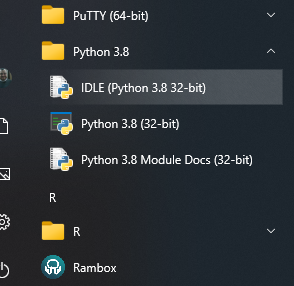
\includegraphics[scale=0.7]{Imagenes/Guia_IDE_06.png}
    \caption{Lanzamos el IDLE en el menú de Programas en Windows.}
\end{figure}
Escribimos el código como lo hemos considerado, se nos muestra un resaltado de texto en colores, así como hay un autocompletado para ciertas funciones incluidas.
\begin{figure}[H]
    \centering
    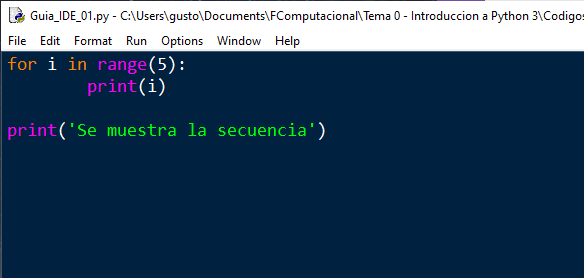
\includegraphics[scale=0.7]{Imagenes/Guia_IDE_07.png}
    \caption{El código dentro del archivo.}
\end{figure}
Se debe de guardar el archivo con la respectiva extensión \texttt{.py}, para ejecutar el código en Windows presionamos la tecla \keys{F5}, abriéndose otra ventana con el resultado.
\begin{figure}[H]
    \centering
    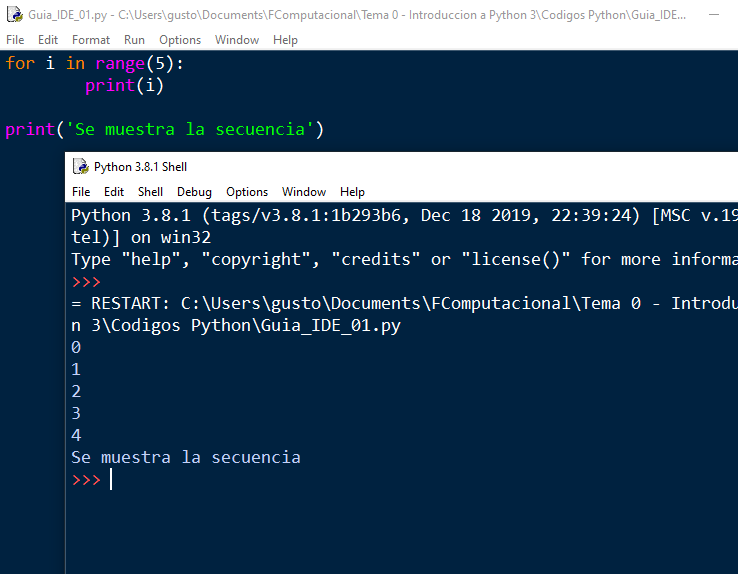
\includegraphics[scale=0.7]{Imagenes/Guia_IDE_08.png}
    \caption{Ventana del entorno de \python{} con el resultado del código.}
\end{figure}

\subsection{Los IDE para programar.}

Un entorno de desarrollo integrado (\textbf{IDE}) es un programa para el diseño y desarrollo de aplicaciones que combina herramientas comunes para programadores en una sola interfaz de usuario gráfica (\textbf{GUI}).
\par
Generalmente, un IDE cuenta con lo siguiente:
\begin{enumerate}[label=\alph*)]
\item \textit{Editor de código fuente}: es un editor de texto que ayuda a escribir el código, cuenta con  con funciones como el resaltado de la sintaxis con indicaciones visuales (colores), el completado automático específico para el lenguaje y la comprobación de errores a medida que se escribe el código.
\item \textit{Terminal}: se incluye una terminal dentro del IDE, por lo que es posible mediante comandos, ocupar la terminal no solo para ejecución, sino para otras tareas: crear carpetas, copiar, mover, eliminar archivos, etc. Los IDE vinculan la ejecución del código de manera automática, es decir, no será necesario escribir la instrucción para ejecutar un código en \python.
\item \textit{Depurador}: es un programa que sirve para probar los programas que estamos generando y mostrar la ubicación de un error en el código original de forma gráfica, así como hacer una inspección de las variables que estamos utilizando en el código.
\item \textit{Explorador de archivos}: podemos ubicar archivos dentro del mismo IDE, permitiendo su lectura: ya sean imágenes, texto, datos, etc.
\item \textit{Gráficas}: contiene un espacio para visualizar las gráficas que se generen, permitiendo una manipulación básica sobre la gráfica, así como para guardar la imagen.
\end{enumerate}

Existen varios IDE para programar con \python y con otros lenguajes bajo licencia GNU, entre ellos tenemos:
\begin{enumerate}[label=\roman*)]
\item Spyder.
\item Eclipse.
\item Netbeans.
\item Geany.
\item PyDev.
\item Visual Studio Code.
\end{enumerate}

Los IDE de pago (licencia) más comunes para trabajar con \python{} son:
\begin{enumerate}[label=\alph*)]
\item PyCharm.
\item Sublime Text.
\end{enumerate}

Aunque hay que señalar que en el caso de PyCharm, cuenta con dos versiones: a): \textit{Professsional}, que incorpora el soporte y manejo de otros lenguajes como HTML, CSS, JavaScript y para el manejo de bases de datos SQL o mySQL; b): \textit{Community}, que cuenta con todas las funcionalidades aunque no la integración de los lenguajes mencionados previamente.
\par
La versión de uso de Sublime Text, permite la operación completa del programa, mostrando ocasionalmente un mensaje para comprar la licencia, que suele ser un distractor hasta que se paga y el mensaje desaparece.

\subsection{¿Cuál es el mejor IDE?}

Esta respuesta está en función de tus gustos, del modo que prefieras trabajar, ya que algunos editores son muy propios de la programación desde terminal, otros que tienen una interfaz gráfica que facilita el trabajo.
\par
Cada IDE permite una configuración desde la apariencia (temas, íconos, etc.) así como la instalación de plugins para extender la funcionalidad del mismo.
\par
Se recomienda elegir un IDE para dedicarle el tiempo de estudio, revisando la documentación oficial y profundizar en el manejo del programa, de esta manera se enfocarán al trabajo de programación con \python{} con una herramienta adicional. En el curso usaremos \textbf{Spyder} como IDE, además de que viene incluido en la suite de \textit{Anaconda-Navigator}.

\section{Spyder.}

\textbf{Spyder} es de código abierto, es un IDE para el desarrollo de \python{} con un orientación de cómputo científico, en contraste \textbf{PyCharm} es de carácter más general, ya que permite el desarrollo de aplicaciones de escritorio, de terminal, web, interfaces visuales, conexión con bases de datos, etc.
\par
\textbf{Spyder} es el acrónimo en inglés \enquote{\textbf{S}cientific \textbf{PY}thon \textbf{DE}veloment envi\textbf{R}onment}, su interfaz de usuario está bien planificada ya que cuenta con opciones interactivas, diseños personalizables y secciones intercambiables.
\par
Algunas de las características \textbf{Spyder} son:
\begin{enumerate}[label=\alph*)]
\item Es multiplataforma: hay una versión para Linux, Windows y iOS.
\item Es de código gratuito y abierto.
\item Resalta la sintaxis.
\item Cuenta con completado de instrucciones.
\item Tiene una consola interactiva.
\item Incluye un explorador de variables.
\item Tiene un visor de documentación, visualización de gráficos y datos.
\end{enumerate}

\subsection{El entorno de Spyder.}

Del menú de aplicaciones de \textit{Anaconda-Navigotor} localizamos el ícono de Spyder para \enquote{lanzarlo}:
\begin{figure}[H]
    \centering
    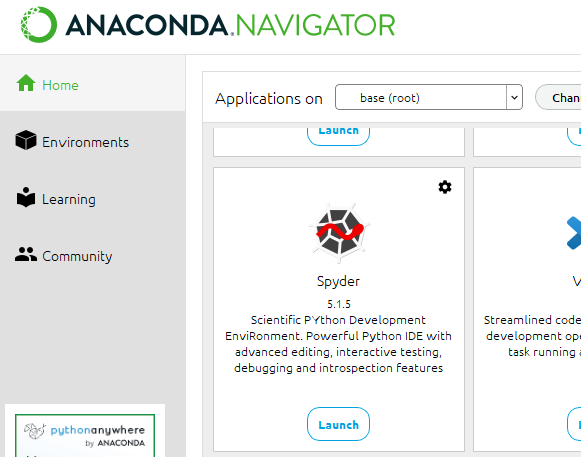
\includegraphics[scale=0.5]{Imagenes/Guia_IDE_09.png}
\end{figure}
Tendremos abierta una ventana con tres secciones que revisaremos a continuación:
\begin{figure}[H]
    \centering
    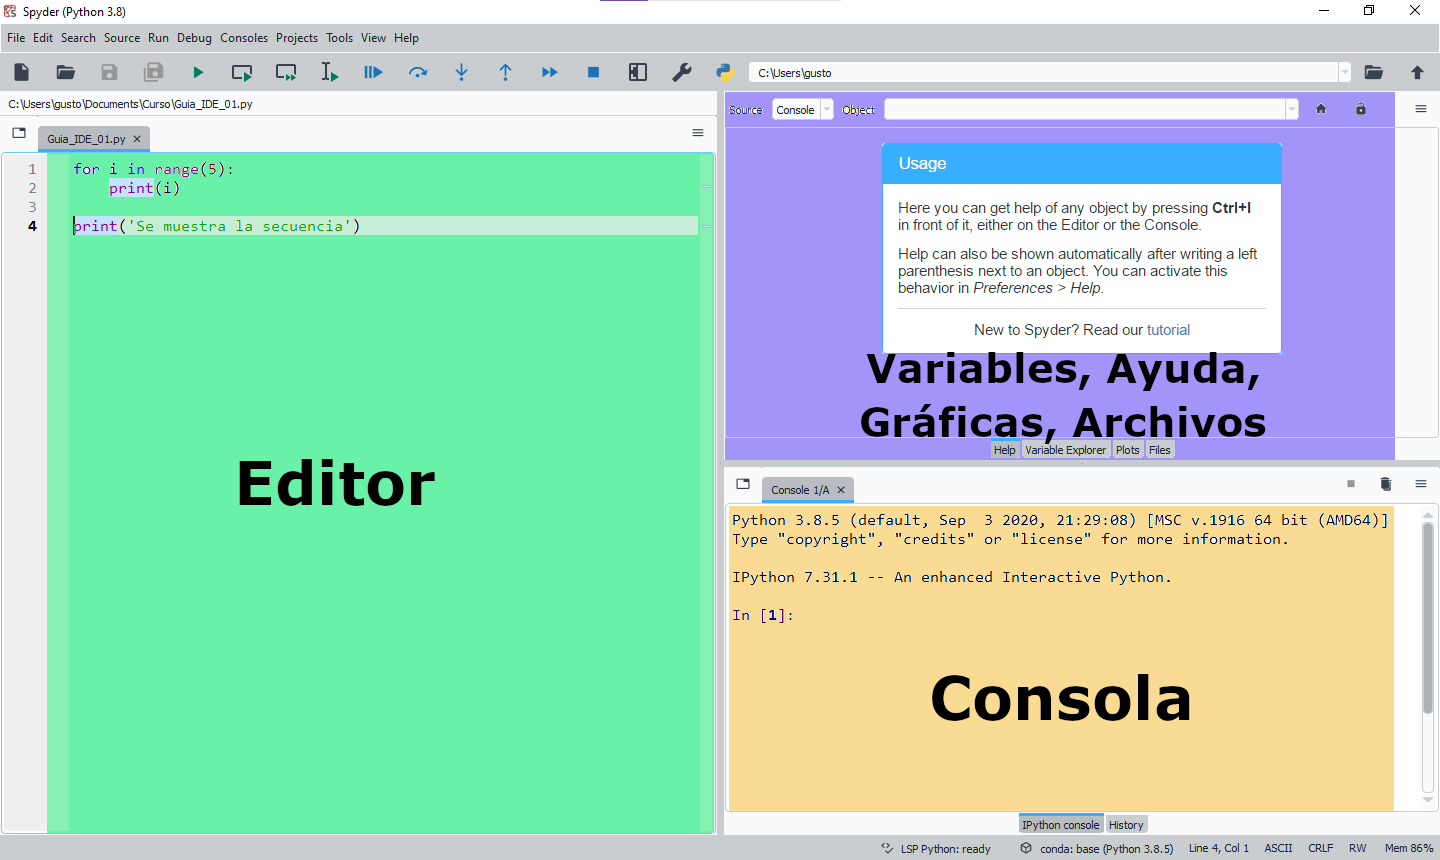
\includegraphics[scale=0.4]{Imagenes/Guia_IDE_10.png}
\end{figure}

\subsection{El Editor.}

El panel del \textit{Editor} de Spyder es el elemento clave del IDE, ya que soporta varios lenguajes y es donde puede crear, abrir y modificar archivos de código. El Editor ofrece una variedad de funciones básicas, como autocompletado, análisis en tiempo real, resaltado de sintaxis, división horizontal y vertical, y mucho más. Además, integra una serie de potentes herramientas para una experiencia de edición eficiente y fácil de usar.
\par
El Editor se compone de varias partes como podemos ver en la siguiente figura:
\begin{figure}[H]
    \centering
    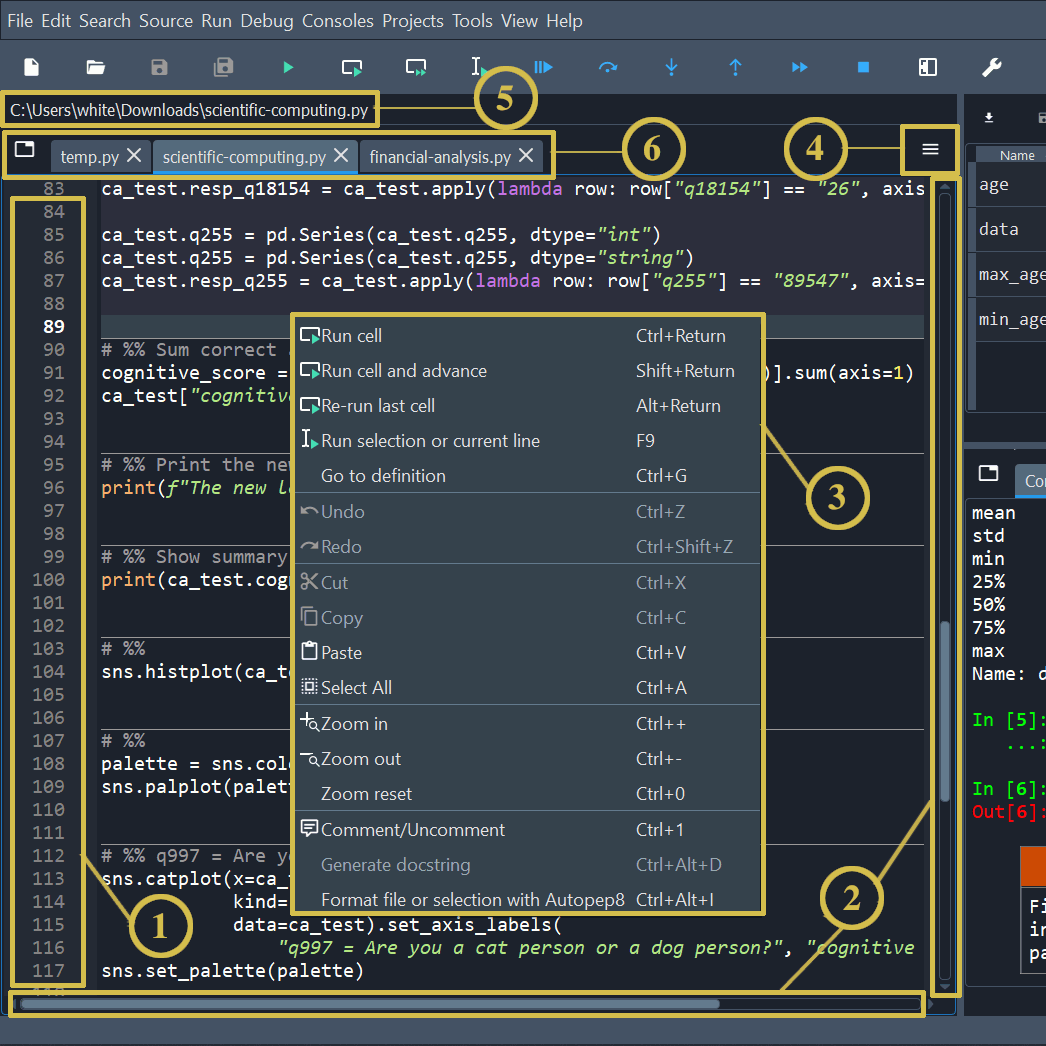
\includegraphics[scale=0.25]{Imagenes/Guia_IDE_11.png}
\end{figure}
De la figura anterior tenemos los elementos:
\begin{enumerate}
\item  La barra lateral izquierda muestra los números de línea y muestra las advertencias de análisis de código que existen en el archivo actual. Al hacer click en un número de línea, se selecciona el texto en esa línea y al hacer click a la derecha se establece un punto de interrupción.
\item Las barras de desplazamiento permiten la navegación vertical y horizontal en un archivo.
\item El menú contextual (click con el botón derecho del ratón) muestra acciones relevantes para lo que se haya hecho click.
\item El menú de opciones (ícono \enquote{Hamburguesa} en la parte superior derecha) incluye configuraciones y acciones útiles relacionadas con el Editor.
\item La barra de ubicación en la parte superior del panel Editor muestra la ruta completa del archivo actual.
\item La barra de pestañas muestra los nombres de todos los archivos abiertos. También tiene un botón Examinar pestañas (a la izquierda) para mostrar todas las pestañas abiertas y cambiar entre ellas, lo que resulta útil si hay muchas abiertas.
\end{enumerate}

\subsection{La consola.}

En esta ventana veremos la ejecución del archivo y el resultado en la terminal, aquí se mostrarán los mensajes de error en caso de que se presente alguno.
\par
En esta ventana podemos interactuar con el código si deseamos ingresar un valor para que se procese dentro del algoritmo.

\subsection{Multiventanas.}

En la parte superior derecha tenemos un espacio para distintas tareas:
\begin{enumerate}[label=\alph*)]
\item \textit{Ayuda}: Si buscamos el soporte dentro de la documentación de \python, podemos recurrir a esta ventana para visualizar la ayuda en específico: seleccionamos la instrucción de interés, y presionamos la combinación de teclas \keys{\ctrl} + \keys{I}, lo que nos mostrará la información sobre nuestra consulta.
\item \textit{Explorador de variables}: Podemos hacer un seguimiento del contenido de las variables durante la ejecución del código, a esta tarea se le conoce como \textit{debugging} (en español, depuración). Esta tarea nos permite identificar y corregir errores, Spyder cuenta con un modo de depuración que reconoce los puntos de interrupción que se indican dentro del Editor de código, la revisión se hace instrucción por instrucción, encontrando los valores que toman las variables en esta ventana.
\item \textit{Plots}: En esta pestaña se mostrarán las gráficas que hayamos generado con el código, en caso de que sean varias, se presentará a modo de lista. Recomendamos \enquote{separar} las gráficas en una ventana aparte, esto lo logramos dentro de las preferencias de Spyder, en la barra de menú buscamos:
\begin{center}
\menu[,]{Tools, Preferences, IPyhton Console, Graphics, Completion Type}
\end{center}
donde se debe de dejar la opción de la lista en \textit{Automatic.}
\item \textit{Explorador de archivos}: Donde podemos localizar la carpeta y archivos de trabajo, que podemos abrir ya sean códigos de \python, archivos de texto plano, incluso imágenes.
\end{enumerate}

\section{Recursos para Spyder.}

Lo más recomendable para aprender a utilizar el IDE Spyder, es revisar en la página web la \href{https://www.spyder-ide.org/}{documentación oficial}, que además de presentar un contenido, incluye una serie de tres videos cortos que les serán de utilidad, los videos están en inglés pero es entendible ya que no es tan técnico, por lo que queda en ustedes ampliar la información para que obtengan el mayor provecho de este entorno de trabajo para \python.

\subsection{Lista de videos.}

Al hacer click sobre la liga, te enviará al video dentro del canal de YouTube de Spyder.

\begin{enumerate}
\item Parte 1. Comenzando con Spyder. \href{https://youtu.be/E2Dap5SfXkI}{\texttt{https://youtu.be/E2Dap5SfXkI}}
\begin{figure}[H]
    \centering
    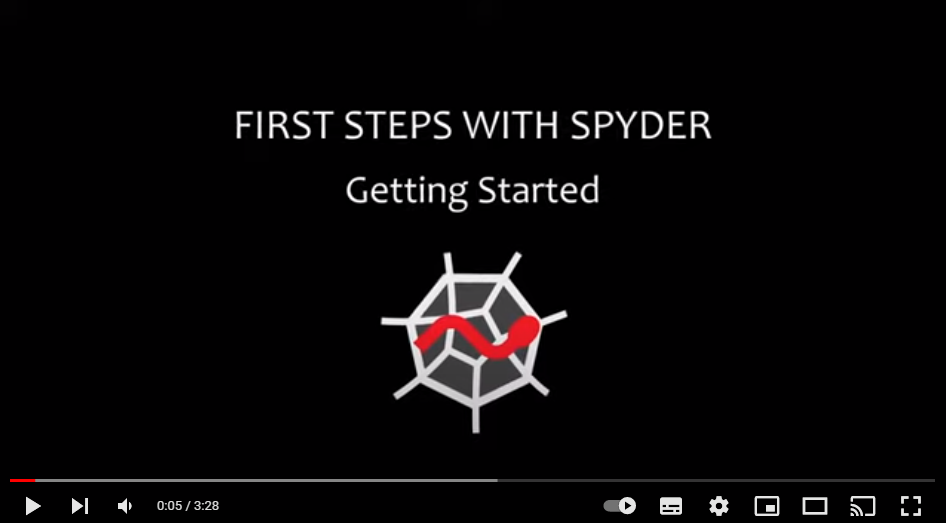
\includegraphics[scale=0.4]{Imagenes/Guia_IDE_12.png}
\end{figure}
\item Parte 2. Aprendiendo lo básico. \href{https://youtu.be/WV9bm4ey7Cg}{\texttt{https://youtu.be/WV9bm4ey7Cg}}
\begin{figure}[H]
    \centering
    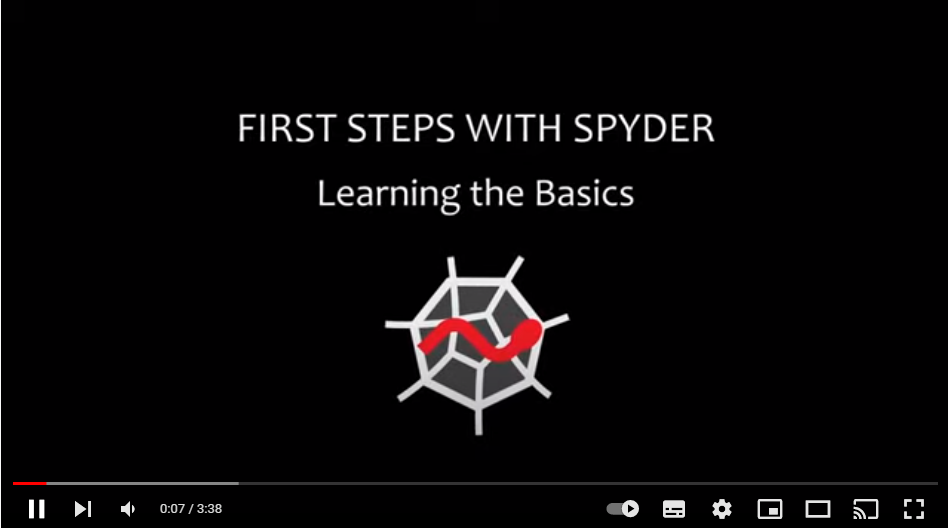
\includegraphics[scale=0.4]{Imagenes/Guia_IDE_13.png}
\end{figure}
\item Parte 3. Personalización. \href{https://youtu.be/-dARZBUDk_s}{\texttt{https://youtu.be/-dARZBUDk\_s}}
\begin{figure}[H]
    \centering
    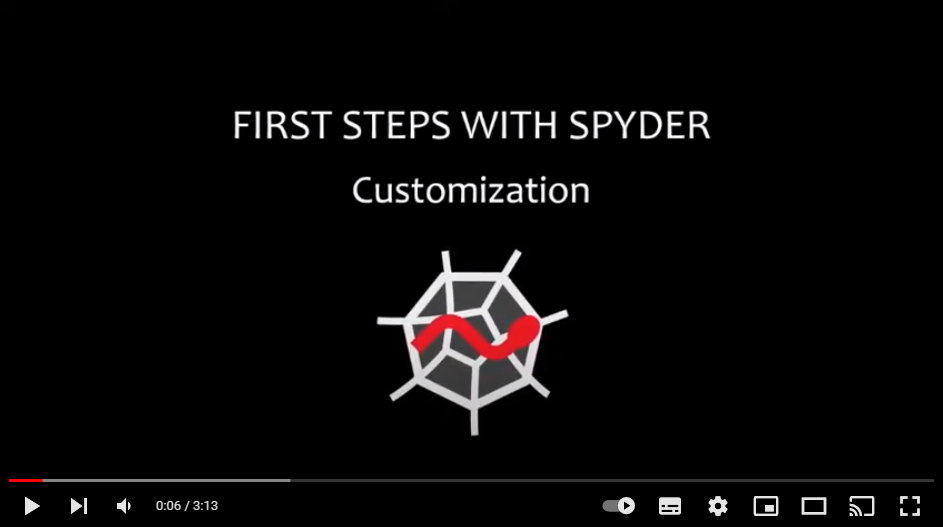
\includegraphics[scale=0.4]{Imagenes/Guia_IDE_14.png}
\end{figure}
\end{enumerate}

\end{document}

